\documentclass[tikz,border=8pt]{standalone}
\usetikzlibrary{arrows.meta,positioning}
\begin{document}
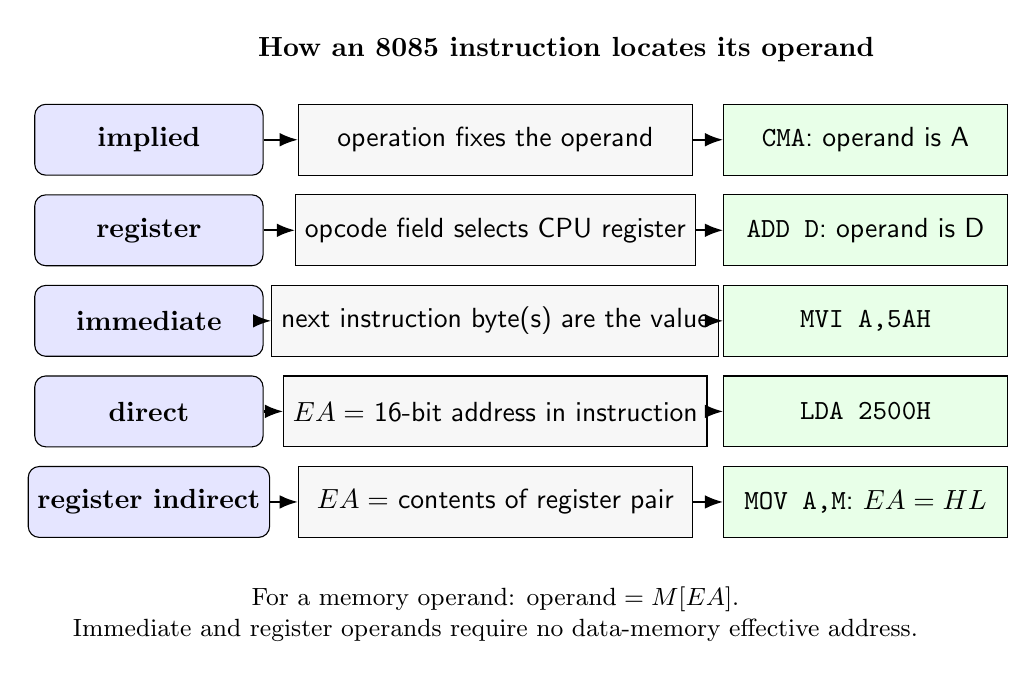
\begin{tikzpicture}[
  font=\sffamily,
  >=Latex,
  mode/.style={draw,rounded corners,fill=blue!10,minimum width=2.9cm,minimum height=0.9cm,align=center,font=\bfseries},
  rule/.style={draw,fill=gray!6,minimum width=5.0cm,minimum height=0.9cm,align=center},
  example/.style={draw,fill=green!9,minimum width=3.6cm,minimum height=0.9cm,align=center},
  flow/.style={->,thick}
]
\node[font=\bfseries] at (5.3,3.35) {How an 8085 instruction locates its operand};

\node[mode] (m1) at (0,2.2) {implied};
\node[rule] (r1) at (4.4,2.2) {operation fixes the operand};
\node[example] (e1) at (9.1,2.2) {\texttt{CMA}: operand is A};

\node[mode] (m2) at (0,1.05) {register};
\node[rule] (r2) at (4.4,1.05) {opcode field selects CPU register};
\node[example] (e2) at (9.1,1.05) {\texttt{ADD D}: operand is D};

\node[mode] (m3) at (0,-0.10) {immediate};
\node[rule] (r3) at (4.4,-0.10) {next instruction byte(s) are the value};
\node[example] (e3) at (9.1,-0.10) {\texttt{MVI A,5AH}};

\node[mode] (m4) at (0,-1.25) {direct};
\node[rule] (r4) at (4.4,-1.25) {$EA=$ 16-bit address in instruction};
\node[example] (e4) at (9.1,-1.25) {\texttt{LDA 2500H}};

\node[mode] (m5) at (0,-2.40) {register indirect};
\node[rule] (r5) at (4.4,-2.40) {$EA=$ contents of register pair};
\node[example] (e5) at (9.1,-2.40) {\texttt{MOV A,M}: $EA=HL$};

\foreach \n in {1,...,5}{
  \draw[flow] (m\n) -- (r\n);
  \draw[flow] (r\n) -- (e\n);
}
\node[below=5mm of r5,font=\small,align=center] {For a memory operand: $\mathrm{operand}=M[EA]$.\\Immediate and register operands require no data-memory effective address.};
\end{tikzpicture}
\end{document}
